\section{Background}
\label{sec:background}

\subsection{Coherent Combining in Distributed MIMO}
\label{sec:simo}

\begin{figure}[htb]
    \centering
    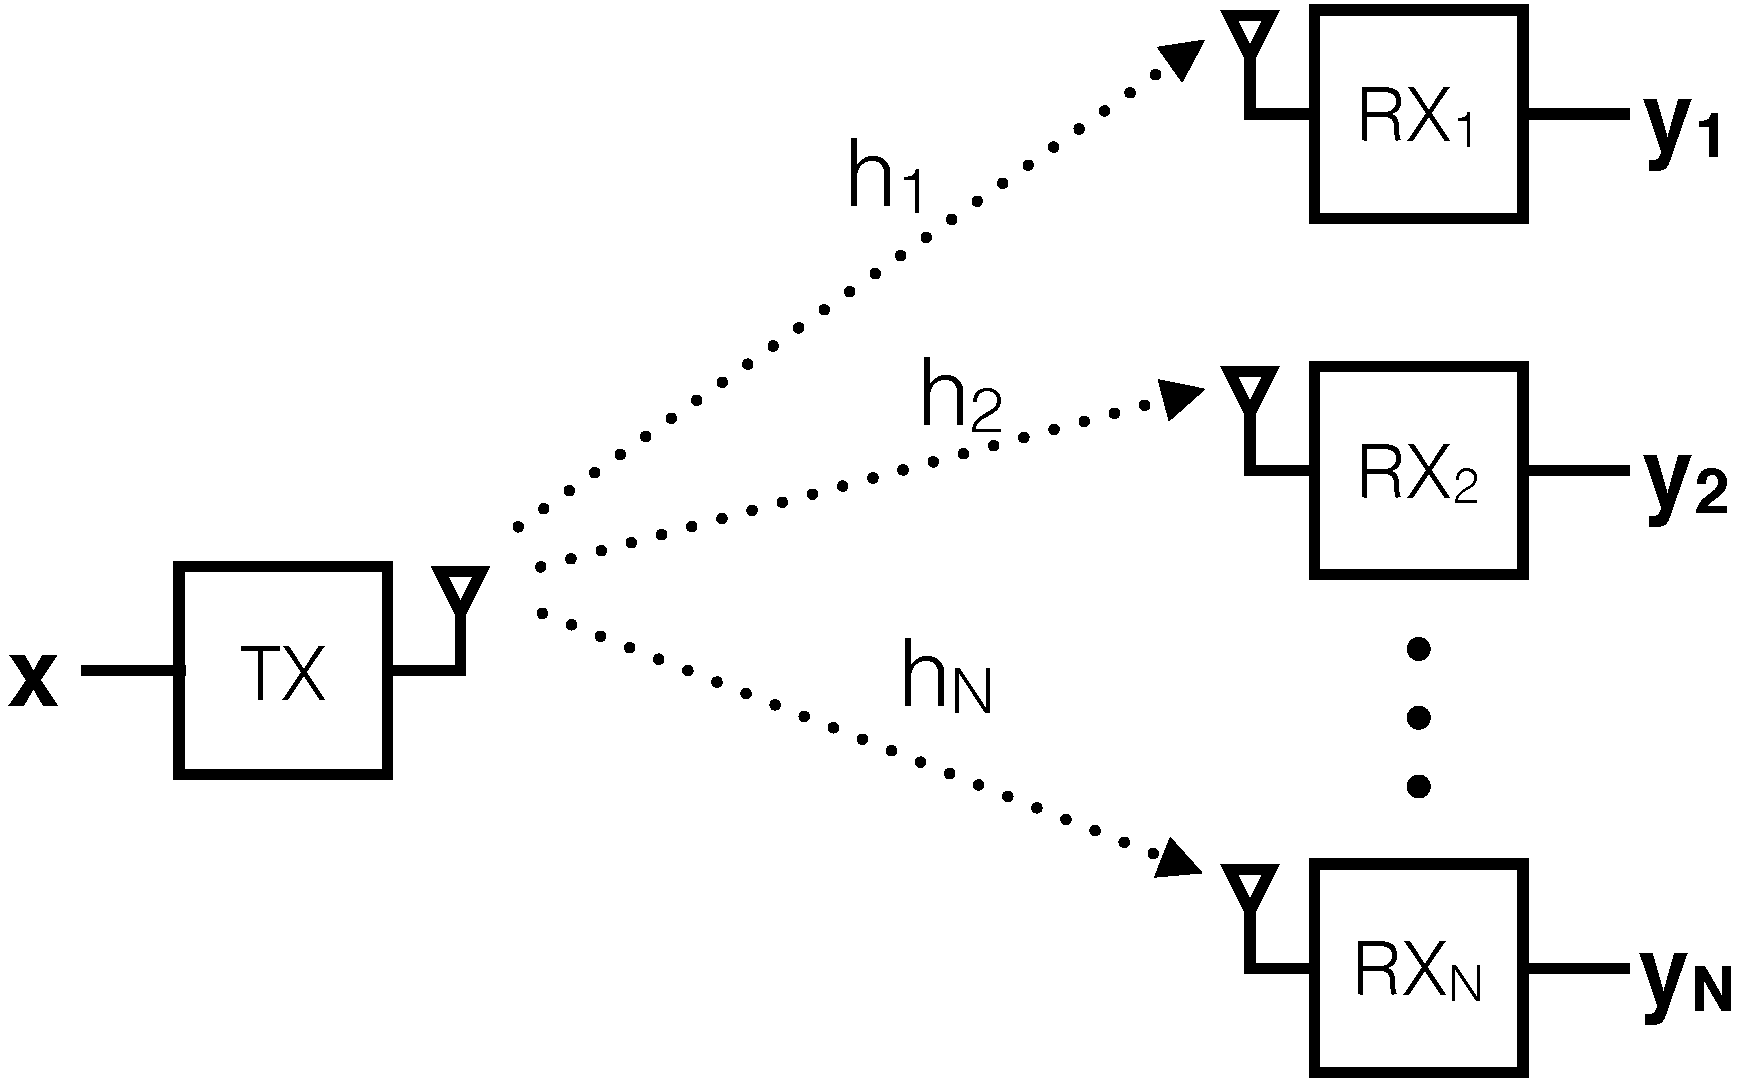
\includegraphics[height=1.25in]{figures/SIMO_cropped}
    \caption{Coherent combining helps receivers collaboratively improve
        signal-to-noise ratio}
    \label{fig:simo}
    \compactimg
\end{figure}

Wireless radios leverage multiple antennas (MIMO or multiple-input
multiple-output) to improve throughput. This paper considers coherent
combining where transmissions from a single-antenna transmitter (e.g. an
LP-WAN client) are heard by multiple receiver antennas (e.g. LP-WAN gateways).
These gateways can then coherently combine the received signals to improve
signal decodability.

Mathematically, let the transmitted signal be $x$ and each of the gateways
receive a signal $y_i$ through wireless channel $h_i$, introducing an
independent noise $n_i$ at the receivers. For a narrow-band system (as is
LoRaWAN and most LP-WAN technologies), we can write the received signal as:
$y_i = h_i x_i + n_i $.

The receivers can now coherently combine their received signals by using the
known wireless channels $h_i$:

\begin{align*}
y_{\text{combined}}
	= \sum_{i=1}^N h^*_i y_i
	= \sum_{i=1}^N \left| h_i \right|^2 x + \sum_{i=1}^N h^*_i n_i
\end{align*}

The first term is the combined signal while the second term is the combined
noise. However, while the signals add up coherently, the noise, being
independent, adds up incoherently.  This results in an overall increase in the
combined signal-to-noise ratio (SNR) which allows us to jointly decode a
packet that may otherwise not be decodable by any individual receiver.

\begin{align*}
SNR_{\text{combined}} %= \frac{\text{total signal power}}{\text{total noise power}} 
	= \frac{\left| \sum_{i=1}^N \left| h_i \right|^2 x \right|^2}{\sum_{i=1}^N \left| h^*_i n_i \right|^2} 
	\geq \frac{\left| \left| h_i \right|^2 x \right|^2}{\left| h^*_i n_i \right|^2} = SNR_i
\end{align*}

In practice, performing coherent combining as shown above makes two important
assumptions: (1) the packets can be detected at individual receivers above
some SNR threshold, and (2) receivers share a common clock reference for time
and frequency. This paper describes the challenges in implementing coherent
combining in the low-power wide-area context where neither assumption holds.


\subsection{Primer on LoRaWAN PHY and MAC}
\label{sec:lora}

LoRaWAN is a popular LP-WAN technology that operates in the sub-GHz ISM band
(900 MHz in the U.S.) and bandwidths of 125-500kHz. LoRaWAN clients can
transmit at low-data rates (few kbps) to gateways up to 10 km away in free
space and last up to 10 years on AA batteries. Below, we detail a few key
design decisions of LoRaWAN.

\noindent \textbf{LoRa, The PHY: } LoRa's physical layer is based on
chirp-spread spectrum modulation, i.e. using a chirp signal that continuously
varies in frequency. This makes it resilient to interference, multi-path
fading and doppler effects. Every LoRaWAN packet begins with a preamble of
sixteen repeated chirps followed by data. Each data chirp encodes multiple
data bits (more precisely, \textit{chips}), with the number of  bits encoded
per chirp called the \textit{spreading factor} (SF). For instance, at
spreading factor of seven, each chirp encodes 7 bits with $2^7 = 128$ possible
uniformly separated initial frequencies. A higher spreading factor, e.g.
eight, encodes one more bit per chirp but also incurs double the transmission
time, effectively halving the data rate.\footnote{More precisely, increasing
spreading factor from $n$ to $n+1$ scales data rate by $(n+1)/2n$.} Increased
spreading factors are used to simultaneously slow down transmissions and
improve resilience to noise. LoRaWAN radios are therefore designed to transmit
at the lowest possible spreading factor that can be received at existing noise
levels for minimizing transmission time and the resulting battery drain. This
paper therefore strives to reduce spreading factor (improve data rate) for
weak transmitters.

\vspace*{0.02in}

\noindent \textbf{The MAC: } LoRaWAN networks are designed to be simple
star-topologies that have client devices directly communicating with a gateway
that is connected to the internet over ethernet or cellular links. Gateways
are simple and relatively inexpensive forwarders that send received packets to
a cloud LoRaWAN server, and can be commanded by the server to transmit data to
clients at a specific time. Packet decoding, managing acknowledgements and MAC
parameters like data-rate are decided at a LoRaWAN server. The LoRa community
often refers to the system as having a ``MAC-in-the-Cloud'' design. LoRaWAN
allows and encourages its users to deploy their own gateways. These gateways
are completely unplanned and on low-bandwidth, unreliable internet connections
(compared to cellular base-stations that are extensively planned and have
dedicated optic fiber connections). In this paper, we refer to these as
user-deployed gateways. The penultimate goal of this paper is to make
individual unreliable user-deployed gateways more valuable by pooling together
PHY-layer processing at the cloud.
